\section{Análisis de Estructuras de Datos}
Como vimos en la sección de Desarrollo, la matriz A vale: \\

\begin{equation*}
A_{ij} = \left\{
  \begin{array}{cl}
  \frac{1}{n_{j}} & \text{si hay un link de } j \text{ a } i,\\
  0 & \text{en caso contrario.}\\
  \end{array} \right.
\end{equation*}

Por tal razón, la matriz A puede poseer varios valores nulos dependiendo la instancia del problema. Dado el contexto del problema, entendemos que la cantidad de links de una a página a otras es mucho menor que la cantidad de paginas totales, por lo que varias posiciones valdrán cero. Dado esta característica, queremos analizar si podemos aprovecharla tanto para el aspecto espacial como para el aspecto temporal. 

\subsection{Propuestas}
Analizamos las distintas alternativas para almacenar la matriz esparsa en términos de eficiencia espacial, comparando en qué casos una alternativa es mejor que otra. Tenemos 4 posibles estructuras de datos para almacenar la matriz. Las opciones propuestas son: \\

\begin{itemize}
	\item \textbf{Vector}: Consiste en almacenar la matriz en un único vector del tamaño de la matriz, almacenando todos los valores de la misma incluyendo los valores nulos.  
	\item \textbf{Dictionary Of Keys (DOK)}: Consiste en almacenar los valores de la matriz que no son nulos en un diccionario, donde las \textit{keys} son la dupla fila y columna, y el \textit{value} es el valor en esa posición. Si una posición no se encuentra en el diccionario, significa que el valor en esa posición es cero.
	\item \textbf{Compressed Sparse Row (CSR)}: Consiste en utilizar 3 \textit{arrays}, uno para guardar todos los valores distintos de cero, otro para guardar la columna donde se encuentran los elementos anteriores, y por último uno donde se almacenan los índices de el primer elemento distinto de cero para cada fila.
	\item \textbf{Compressed Sparse Column (CSC)}: Es igual al CSR, sólo que en lugar de almacenar por filas, se almacena por columnas. El primer \textit{array} guarda los mismos valores pero por columnas, el segundo indica la fila de cada elemento y el último indica el primer elemento distinto de cero de cada columna. La cantidad de memoria que utiliza es exactamente la misma que CSR, dado que los dos primeros $arrays$ tienen igual tamaño (la cantidad de elementos no nulos), y al ser la matriz cuadrada, la cantidad de filas es igual a la de las columnas, coincidiendo así el tamaño del tercer $array$.
\end{itemize}

Para el análisis espacial, optamos por utilizar los valores reales de tamaño que se utiliza en C++, dado que realizando un análsis teórico se llegan a conclusiones que no se corresponden con la implemetación. Un ejemplo sería pensar que una lista de $n$ elementos de tamaño $size\_of\_element$ ocupa un tamaño de $n*size\_of\_element$, cuando en realidad, dependiendo de la implementación, es necesario también tener en cuenta el costo espacial de los punteros para la lista. Si esto no es tenido en cuenta, se podría optar por una estructura de datos que en realidad ocupe más espacio del pensado comparado contra otras alternativas. \\
Para los indices utilizamos el tipo $int$, cuyo tamaño es de 4 bytes, mientras que para los valores almacenados en la matriz utilizamos el tipo $double$ cuyo tamaño es 8 bytes. Para los indices se podría utilizar como alternativa \textit{unsigned int}, que también tienen un tamaño de 4 bytes.\\
Definimos \textbf{NNZ} (NonZero) como la cantidad de valores no nulos de la matriz y $n$ la cantidad de filas (coincidente con las columnas dado que es cuadrada). \\

\subsection{Análisis Espacial:}
Para todos los casos, se midió la cantidad de memoria reservada utilizando \textit{valgrind}. Utilizamos para cada caso un pequeño programa que genera una instancia para cada estructura, primero vacía, y luego agregando elementos. De este modo, pudimos observar cuanta memoria utiliza cada estructura por separado. Los resultados del uso de memoria fueron:\\
%http://netlib.org/linalg/html_templates/node91.html

\begin{itemize}
	\item \textbf{Vector}: $n^2 * 8\ bytes$
	\item \textbf{Dictionary Of Keys (DOK)}: $NNZ * 48\ bytes$
	\item \textbf{Compressed Sparse Row (CSR)}: $8*NNZ + 4*NNZ + 4 (n+1)\ bytes$
\end{itemize}

Fue útil tener en cuenta la cantidad de memoria real, principalmente para constatar que tanto Vector como CSR usaran la cantidad teórica estimada, además de saber que DOK utiliza una cantidad mayor a la pensada. Esto se debe a que DOK está implementado sobre el tipo $map$ de C++, que es un Black-Red Tree. Cada elemento cuesta 48 bytes, más que un double ($value$) y dos enteros ($key$), que serían 16 bytes.  \\

Existen casos para los cuales, cada una de las alternativas anteriores es mejor que el resto. Para ejemplificarlo, supongamos que se tiene una matriz con tamaño $n=100$. Graficamos la cantidad de memoria requerida por cada estructura, variando la cantidad de valores distintos de cero: \\ \\

\begin{wrapfigure}{r}{0.6\textwidth}
  \vspace{-20pt}
  \begin{center}
    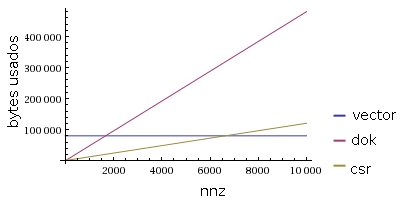
\includegraphics[scale= 0.6]{imagenes/n100espacio.png}
  \end{center}
  \vspace{-20pt}
   \caption[Caption espacio n 100]{Memoria utilizada en una matriz de tamaño 100x100, variando la cantidad de valores no nulos}
  \vspace{-10pt}
  \label{fig:img11}
\end{wrapfigure}

Cabe destacar que, a pesar de no notarse en el gráfico, el Dictionary Of Keys utiliza menos memoria que Compressed Sparse Row para cuando hay menos de 12 valores distintos de cero. A partir de $12 \leq nnz$, Dictionary Of Keys utiliza más memoria. \\ \\ \\ \\  \\
Como conclusión, obtuvimos que Dictionary Of Keys no es una buena alternativa en términos espaciales en comparación a Compressed Sparse Row,  a menos que la matriz fuese sumamente esparsa. La relación entre la cantidad de valores nulos y el tamaño de la matriz para que Dictionary Of Keys presente un mejor desempeño espacial  se detalla en la siguiente tabla.

\begin{center}
    \begin{tabular}{| l | l | l |}
    \hline
    $n$ & $nnz$ & $nnz/n^2$  \\ \hline
    10	& 1	& \%1 \\ \hline
	100	& 11	& \%0.0011 \\ \hline
	1000 & 111	& \%0.0001 \\ \hline
	5000 & 555 & \%0.00002 \\ \hline
	10000 & 1111 & \%0.000001 \\ \hline
	120000 & 13333 & \%0.00000009 \\ \hline
    \end{tabular}
\end{center}

Los valores $nnz$ son la cantidad de valores no nulos que haría que Dictionary Of Keys utilice menos memoria que Compressed Sparse Row. La relación $nnz/n^2$ muestra el porcentaje de valores no nulos con respecto a la matriz total. Como se observa, la relación debe ser muy baja.\\

Vector es la mejor implemetación para cuando la matriz no es esparsa, en particular cuando se cumple la siguiente desigualdad: $$3 nnz > 2n^2 - n + 1$$

De este modo, para nuestro problema, Compressed Sparse Row presenta la mejor opción en términos espaciales para nuestro problema, con excepción de los casos anteriormente vistos cuando la matriz es sumamente esparsa y cuando muy poco esparsa.

\subsection{Análisis Temporal:}
En esta sección, comparamos las estructuras de datos en términos de eficiencia temporal. 
Dentro del contexto del método de la potencia detallado en la sección anterior. En particular, queremos ver si podemos aprovechar la esparcidad de la matriz para obtener  $A (1-c)*x $ del paso 4 del algoritmo. Dado que la matriz posee muchos valores nulos, pretendemos aprovechar esto para que la multiplicación escalar y vectorial resulte más eficiente.\\

Para el caso de Vector, no tenemos una forma de explotar la esparcidad de la matriz, dado que se almacenan todos los valores incluyendo los nulos. Tanto para DOK como para CSR, podemos iterar sobre los valores no nulos de la matriz, y multiplicar cada uno por $(1-c)$. En el caso de DOK, simplemente utilizamos un iterador sobre el $map$ utilizado para este fin, mientras que para CSR, recorremos el vector que almacena los valores no nulos y realizamos la multiplicación. Para ambos casos, la complejidad es $O(nnz)$. \\

Para multiplicar por un vector, para DOK recorremos los valores no nulos de la matriz, obtenemos el indice al que corresponde en la matriz, lo multiplicamos por el valor correspondiente del vector y se lo sumamos al vector que devolvemos. El vector devuelto está inicializado en cero en cada posición.


\begin{algorithmic}[1]
  \Function{Multiplicacion Vectorial DOK}{map A, vector x}
    \State res = []
    \State it = A.begin()
    \While{ it != A.end()}
      \State i = it.posicion_fila
      \State j = it.posicion_columna
      \State res[ i ] += it.value * x[j]
    \EndWhile
    \Return res
  \EndFunction
\end{algorithmic}

Para CSR, también aprovechamos las características de la estructura. Para este caso, recorremos el vector de los indices para multiplicar el valor al que apuntan contra el valor del vector. El procedimiento es similar al de DOK, en cuanto a sólo recorrer los valores no nulos. \\

Para ambos casos, la complejidad es $O(n + nnz)$, dado que se debe inicializar el vector resultante (de tamaño $n$), y luego recorrer los valores distintos de cero de la matriz para multiplicar, mientras que para Vector la complejidad es $O(n^2)$.

\subsection{Cargado de la matriz:}
Realizando mediciones temporales, nos dimos cuenta que para algunas instancias particulares, CSR resultaba especialmente lento. El problema radica en el orden de los ejes de la entrada. Cuando los ejes de la entrada no están ordenados de menor a mayor (primero con respecto al valor $i$ y luego al $j$), lo que sucede es que al insertar un valor nuevo en el vector de datos de CSR, deben moverse los subsiguientes valores de lugar. De este modo, cada vez que hay un valor que debería insertarse $d$ posiciones antes del ùltimo elemento, esos $d$ elementos deben de copiarse a una posicón posterior. Si en particular la entrada estaría ordenada de mayor a menor, se deberían moverse:
\begin{eqnarray}
\sum_{i = 0}^{nnz} i = \frac{nnz(nnz+1)}{2}\label{eq:ecuResize}
\end{eqnarray}
Además de la cantidad de veces que se hace un $resize$ del vector al quedarse sin espacio para agregar elementos. \\

Tanto Vector como DOK no sufren de esta problemática.

\subsection{Conclusiones de Estructuras de Datos:}

Concluimos que, dentro del contexto dado, la mejor opción es CSR dado que presenta la mejor opción en términos de eficiencia espacial para el problema planteado (matrices con cierta esparcidad), pudiendo aprovecharse mejoras temporales para el método de la potencia.\\
Sin embargo, dado el problema del cargado de la matriz, es posible que esta estructura no sea viable. Una opción es realizar un pre-procesaminento para reordenar los datos de entrada del programa. Sino, se puede utilizar DOK para este fin, de manera de insertar todos los elementos de la entrada en el DOK, y luego iterarlos en orden para armar la matriz sobre CSR.\\
Por último, en términos de complejidad temporal, Vector resulta la peor alternativa ya que en todos los casos debe multiplicar por todos los elementos, mientras que DOK y CSR proveen soluciones similares que permiten una mayor eficiencia.
